\documentclass{beamer}
\usepackage[T1]{polski}
\usepackage[polish]{babel}
\usepackage[utf8]{inputenc}
\usepackage[T1]{fontenc}
\usepackage[mediumspace,mediumqspace,Grey,squaren]{SIunits}
\usepackage{graphicx}
\usepackage{filecontents}

%\addbibresource{bibliography.bib}

\setbeamertemplate{bibliography item}{\insertbiblabel}


\graphicspath{ {./images/} }

\begin{document}
\title{Sieci czasu rzeczywistego}   
\author{Jakub Arnold Postępski-Winiarski von Seredyński el Pacuszka} 
\date{\today} 

\frame{\titlepage} 




\frame{\frametitle{Rozkład jazdy}
	\begin{itemize}
		\item Wprowadzenie
		\item Potrzebne narzędzia
		\item Wybrane implementacje sieci RT
		\item Praktyczne realizaje
		\item Podsumowanie
	\end{itemize}
	}
	
\frame{
	
	\frametitle{Definicje}
	\textbf{Systemy czasu rzeczywistego} - 	Urządzenie techniczne, którego wynik i efekt działania jest zależny od chwili wypracowania tego wyniku. \cite{wiki:RTC}\\
	\textbf{Przepustowość} - In computing, bandwidth is the bit-rate of available or consumed information capacity expressed typically in metric multiples of bits per second. Variously, bandwidth may be characterized as network bandwidth, data bandwidth, or digital bandwidth. \cite{wiki:Przepustowosc}
	
}

\frame{
	\frametitle{Co chcemy uzyskać? - Sieci telekomunikacyjne}
	\begin{itemize}
		\item Telekomunikacja
		\item Kontrola systemów infrastruktury
		\item Automotive
		\item Medycyna
		\item Wojsko
		\item Przemysł
		\item Energetyka
		\item Robotyka
	\end{itemize}
}


\frame{\frametitle{Co chcemy łączyć? - Urządzenia}
	\begin{itemize}
		\item Linux z patchem RT
		\item BeagleBone
		\item $\micro$C na przerwaniach
		\item $\micro$C z pseudo systemem operacyjnym
		\item PLC
		\item FPGA
	\end{itemize}
}



\frame{
	\frametitle{Przykład urządzenia}
		\begin{figure}
			\centering
			\includegraphics[width=0.99\linewidth,page=2]{motherboard}
			\caption{Schemat ideowy płyty głównej laptopa \cite{image:motherboard}}
			\label{fig:motherboard}
		\end{figure}
	}


\frame{
	\frametitle{Rodzaje łącz}
	\begin{itemize}
		\item Bezprzewodowe
		\item Przewodowe
		\item Światłowodowe
	\end{itemize}
	\begin{itemize}
		\item Szeregowe
		\item Równoległe
	\end{itemize}
	\begin{itemize}
		\item Analogowe
		\item Cyfrowe
		\item Ze zwielokrotnieniem falowym
	\end{itemize}
}

\frame{
	\frametitle{Problemy z automatycznymi gołąbkami}
	\begin{itemize}
		\item Half duplex
		\item Full duplex
	\end{itemize}
	
	\begin{itemize}
		\item Jeden master
		\item Wiele masterów
		\item Wykrywanie kolizji
		\item Tokeny
		\item Synchronizacja czasu
		\item Enkapsulacja
		\item Kompresja
		\item Korekcja błędów
		\item Zakłócenia elektromagnetyczne
		\item Ilość węzłów w sieci
		\item Skończona prędkość rozchodzenia fali
	\end{itemize}
}

\frame{
	\frametitle{Elektronika}
	\begin{itemize}
		\item $\micro$C
		\item Wzmacniacze
		\item Komparatory
		\item Transformatory
		\item A/C
	\end{itemize}
}


\frame{
	\frametitle{Otwarty kolektor/dren}
	\begin{figure}
		\centering
		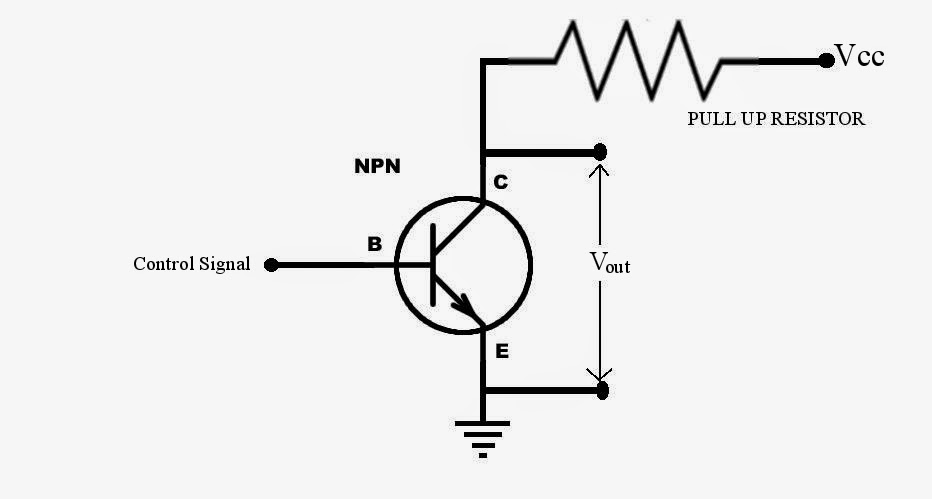
\includegraphics[width=0.9\linewidth]{open_collector}
		\caption{Schemat otwartego kolekotra\cite{image:collector}}
		\label{fig:open_collector}
	\end{figure}
}

\frame{
	\frametitle{Optoizolacja}
		\begin{figure}
			\centering
			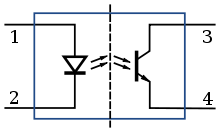
\includegraphics[width=0.9\linewidth]{optoisolation}
			\caption{Schemat transoptora\cite{image:optoisolation}}
			\label{fig:optoisolation}
		\end{figure}
	}

\frame{
	\frametitle{Para różnicowa}
	\begin{figure}
		\centering
		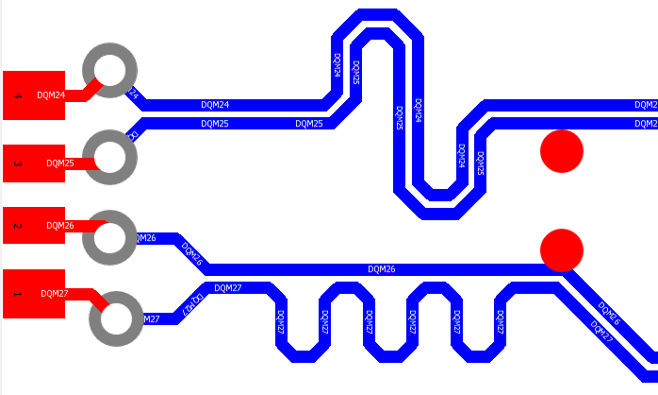
\includegraphics[width=0.9\linewidth]{differential}
		\caption{Przykładowa realizacja pary różnicowej na PCB\cite{image:collector}}
		\label{fig:differential}
	\end{figure}
}

\frame{
	\frametitle{Budowa światłowodu}
	\begin{figure}
		\centering
		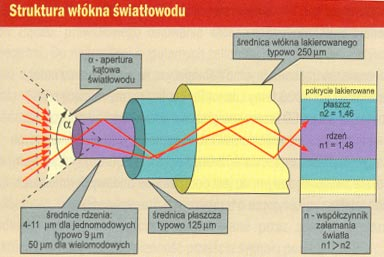
\includegraphics[width=0.9\linewidth]{swiatlowod3}
		\caption{Budowa światłowodu
		\cite{image:swiatlowod}}
		\label{fig:swiatlowod1}
	\end{figure}
}

\frame{
	\frametitle{Rodzaje światłowodów}
		\begin{itemize}
			\item Wielomodowe
			\item Jednomodowe
		\end{itemize}
		
		\begin{itemize}
			\item Skokowe
			\item Gradientowe
		\end{itemize}
		
		\begin{itemize}
			\item Plastikowe
			\item Szklane (np. SiO$_2$)
			\item Półprzewodnikowe (np. GaAs)
		\end{itemize}
	}
	
\frame{
	\begin{figure}
		\centering
		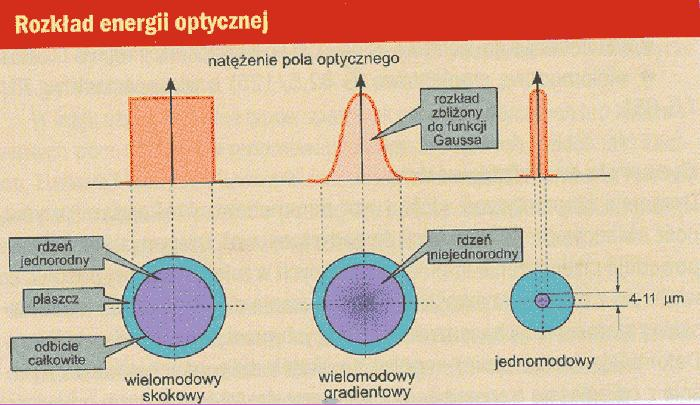
\includegraphics[width=0.9\linewidth]{swiatlowod1}
		\caption{Wyjście światłowodu
			\cite{image:swiatlowod}}
		\label{fig:swiatlowod3}
	\end{figure}
}

\frame{
	\frametitle{Łączenie światłowodu}
	\begin{itemize}
		\item Trwałe
		\item Rozłączne
	\end{itemize}
	
	\begin{figure}
		\centering
		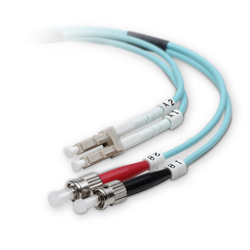
\includegraphics[width=0.5\linewidth]{swiatlowod4}
		\caption{Złącze LC i ST (dół)
			\cite{image:zlacze}}
		\label{fig:swiatlowod4}
	\end{figure}
	
}


\frame{
	\frametitle{Światłowody}
	\begin{itemize}
		\item Prędkości nawet rzędu Tbit/s
		\item Małe tłumienie - duże odległości
		\item Brak problemów elektromagnetycznych (także bezpieczeństwo)
		\item LED lub laser (klasa 1 - bezpieczny; klasa 4 - poparzenia i pożary)
		\item Problemy z fizycznymi połączeniami
		\item Wrażliwość na uszkodzenia
		\item Koszt wykonania
	\end{itemize}
}

\frame{
	\frametitle{RS-232}
	\begin{itemize}
		\item 2 urządzenia
		\item 15 m
		\item Wystarczą 3 przewody
		\item Wybrane prędkości: 50, 9600, 115200, 921600 bit/s 
		\item Tryb asynchroniczny
		\item Tryb synchroniczny
	\end{itemize}
}

\frame{
	\frametitle{RS-232}
		\begin{figure}
			\centering
			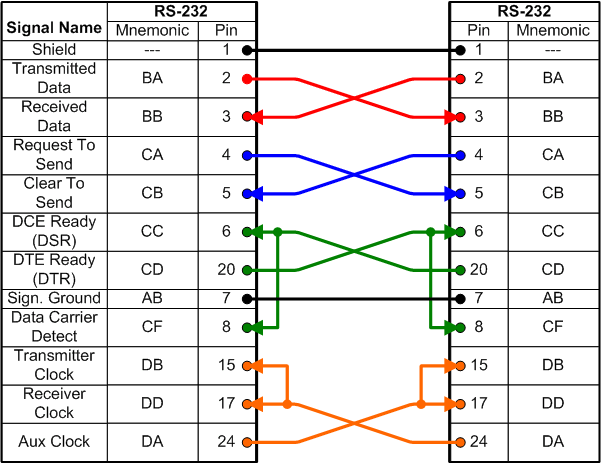
\includegraphics[width=0.9\linewidth]{rs232pin}
			\caption{Piny standardu RS232
				\cite{image:rs232pin}}
			\label{fig:rs232pin}
		\end{figure}
	}

\frame{
	\frametitle{RS-232}
	\begin{figure}
		\centering
		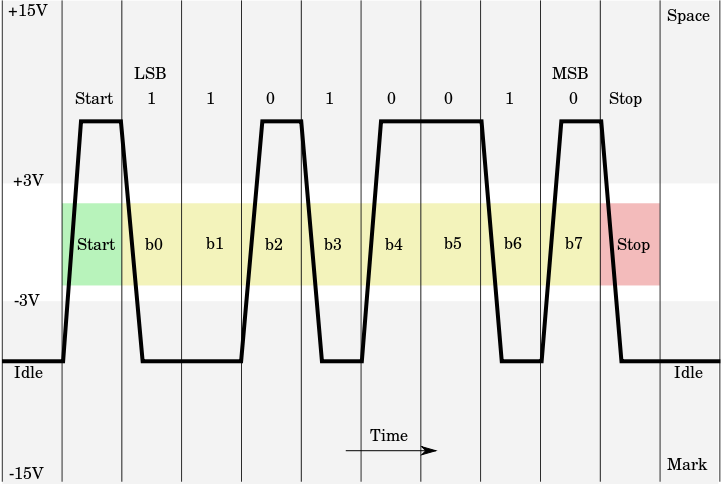
\includegraphics[width=0.9\linewidth]{rs232}
		\caption{Listing przesłania ramki
			\cite{image:rs232}}
		\label{fig:rs232}
	\end{figure}
}


\frame{
	\frametitle{RS-485}
	\begin{itemize}
		\item 32 urządzeń
		\item 1200 m
		\item 10 Mbit/s
		\item Sygnał różnicowy
		\item Half-duplex
	\end{itemize}
	\begin{figure}
		\centering
		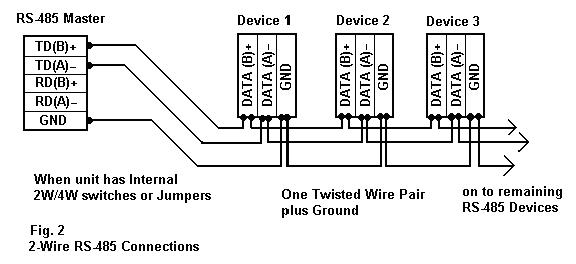
\includegraphics[width=0.7\linewidth]{rs485polaczenie}
		\caption{Schemat połączenia urządzeń
			\cite{image:rs485polaczenie}}
		\label{fig:rs485polaczenie}
	\end{figure}	
}

\frame{
	\frametitle{RS-485 vs RS-232}
	\begin{figure}
		\centering
		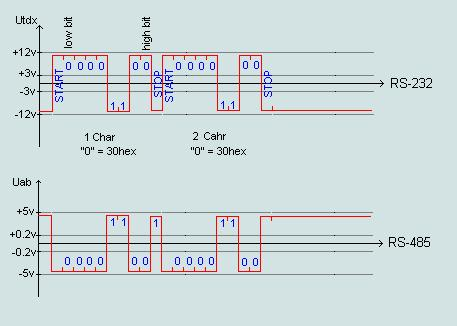
\includegraphics[width=0.9\linewidth]{rs485ramka}
		\caption{Schemat połączenia urządzeń
			\cite{image:rs485ramka}}
		\label{fig:rs485ramka}
	\end{figure}	
}

\frame{
	\frametitle{Modbus}
	\begin{figure}
		\centering
		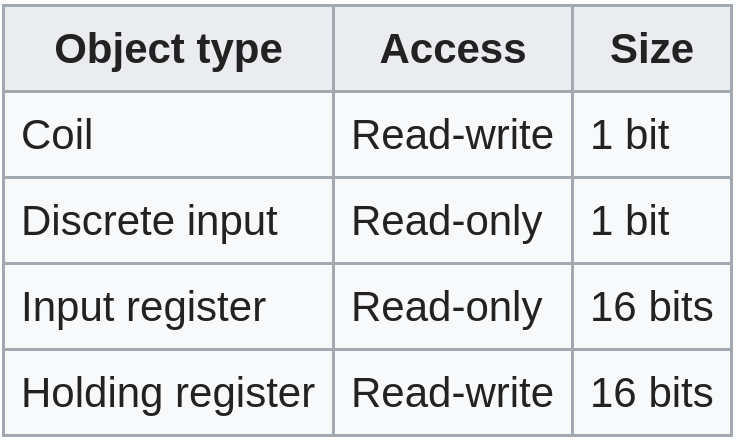
\includegraphics[width=0.4\linewidth]{modbustypy}
		\caption{Typy obiektów
			\cite{image:modbus}}
		\label{fig:modbustypy}
	\end{figure}	
	
	\begin{figure}
		\centering
		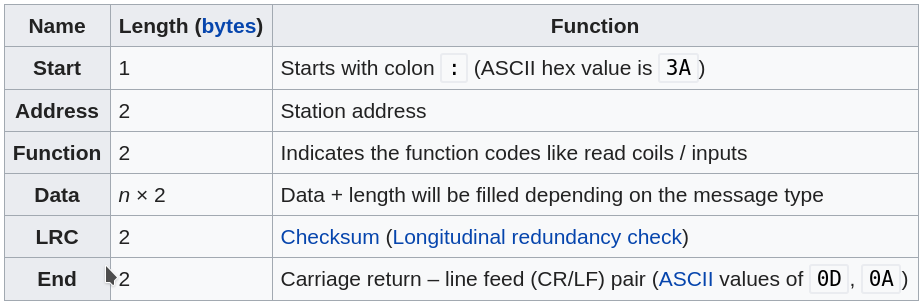
\includegraphics[width=0.9\linewidth]{modbusrtu}
		\caption{Instrukcje protokołu dla RS-485
			\cite{image:modbus}}
		\label{fig:modbusrtu}
	\end{figure}	
}


\frame{
	\frametitle{Modbus}
	\begin{figure}
		\centering
		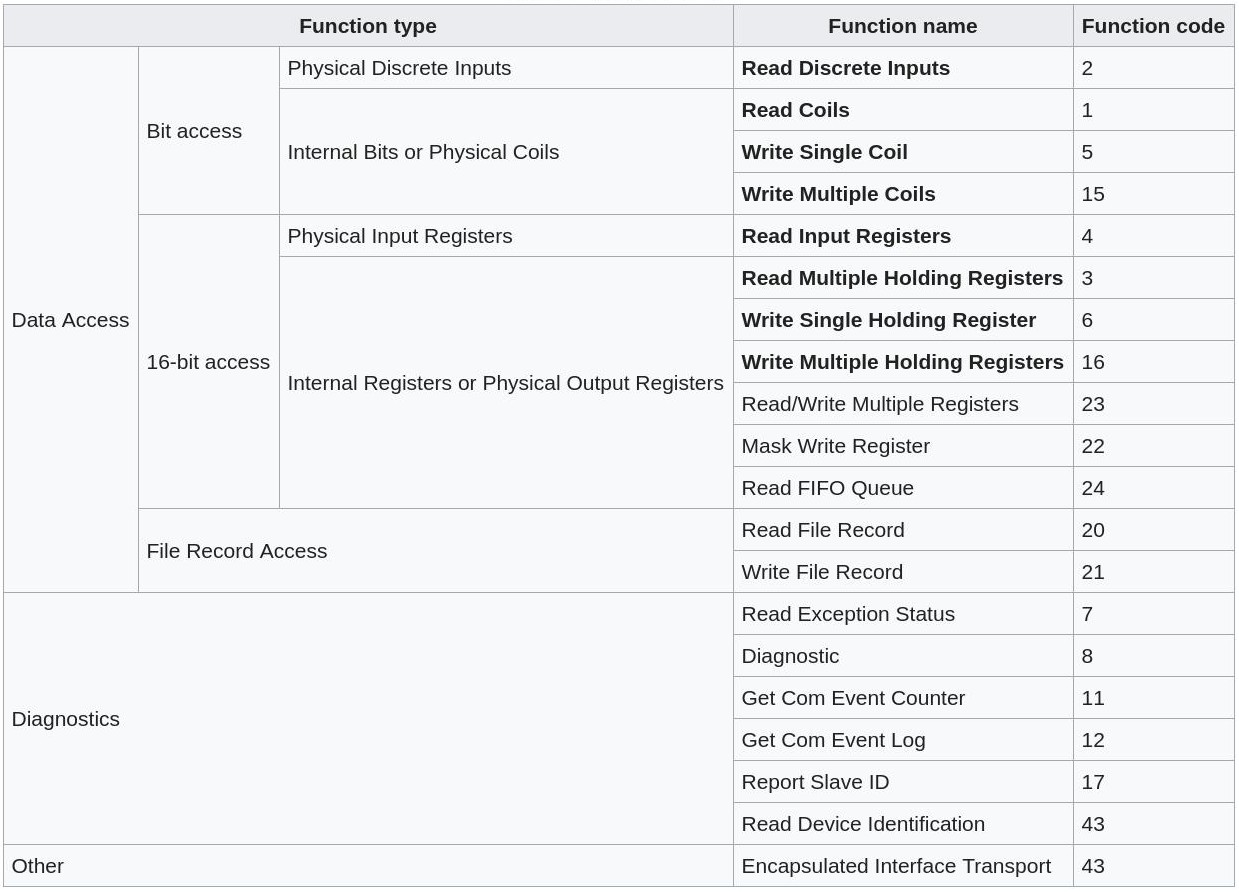
\includegraphics[width=0.9\linewidth]{modbusinstrukcje}
		\caption{Instrukcje protokołu
			\cite{image:modbus}}
		\label{fig:modbusinstrukcje}
	\end{figure}	
}

\frame{
	\frametitle{CAN}
	Stworzona dla automotiwu, ale stosowana szerzej. Niezawodna jak PKiN.
	\begin{itemize}
		\item 40 m
		\item 1 Mbit/s
		\item Równolegle połączona para różnicowa
		\item Specjalne przewody
		\item Rezystory terminalne 120 Ohm
		\item 11 bitowy identyfikator w wersji 2.0A
		\item Multimaster, adresy determinują priorytet
		\item Pull-upy
		\item Zero dominujące
		\item Synchronizacja zegarów (time quanta)
		\item Bit stuffing
		\item Filtrowanie wiadomości
	\end{itemize}
}

\frame{\frametitle{CAN}
		\begin{figure}
			\centering
			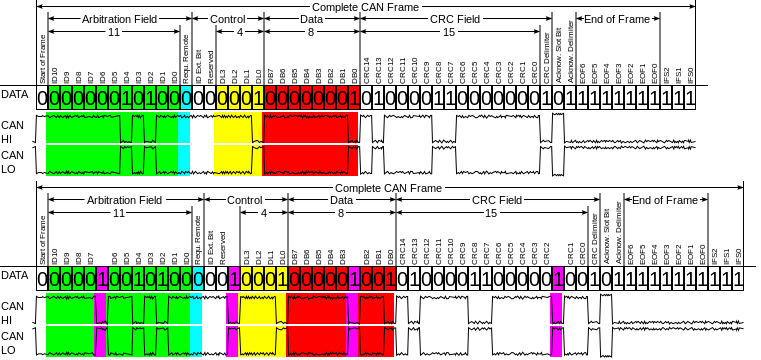
\includegraphics[width=1.0\linewidth]{can}
			\caption{Ramka szyny CAN
				\cite{image:can}}
			\label{fig:can}
		\end{figure}	
	}
\frame{
	\frametitle{CANOpen}
	SDO - Service Data Object:
	\begin{itemize}
		\item Model serwer - klient
		\item Logiczne połączenie 1:1
		\item Możliwość przesyłania danych dowolnego rozmiaru
		\item Konieczność odpowiedzi serwera (może to być błąd)
		\item Narzut protokołu
	\end{itemize}
	PDO - Process Data Object:
	\begin{itemize}
		\item Model producent - konsument
		\item Logiczne połączenie 1:n
		\item Dane długości 8 bajtów
		\item Max. 512 PDO na jedno urządzenie
		\item Wyzwalane zdarzeniem (asynchroniczne)
		\item Wyzwalane wiadomością typu SYNC (synchroniczne)
		\item TxPDO mapping i RxPDO mapping
		\item Mały narzutu protokołu
	\end{itemize}
}
\frame{
	\frametitle{CANOpen}
	NMT - Network Management
	\begin{itemize}
		\item Zmiana stanu urządzenia
		\item Boot-up Message
		\item Node guarding
		\item Heartbeat message
	\end{itemize}
	
	
	LSS - Layer Setting Services (fizyczne połączenie 1:1):
	\begin{itemize}
		\item Przełączenie w tryb
		\item Inquire Node-ID
		\item Configure Node-ID
		\item Configure Bit Timing Parameters
		\item Powrót do trybu zwykłego
	\end{itemize}
}



\frame{
	\frametitle{CANOpen}
	
	\begin{figure}
		\centering
		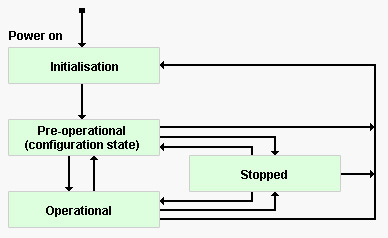
\includegraphics[width=1.0\linewidth]{canstate}
		\caption{Stany urządzenia w sieci
			\cite{image:canstate}}
		\label{fig:canstate}
	\end{figure}
}

\frame{
	\frametitle{CANOpen}
	
	\begin{figure}
		\centering
		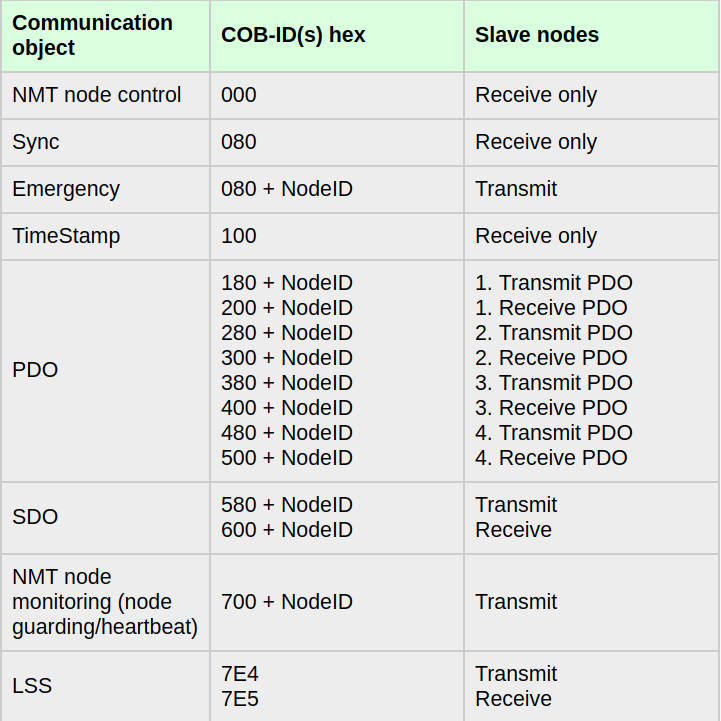
\includegraphics[width=0.7\linewidth]{canopenmap}
		\caption{Przykładowa mapa pamięci rozkazów
			\cite{image:canstate}}
		\label{fig:canopenmap}
	\end{figure}
}

\frame{
	\frametitle{I$^2$C}
	Stosowana do połączeń pojenynczych elementów elektronicznych lub płytek
	\begin{itemize}
		\item Połączenie równoległe
		\item 5 Mbit/s
		\item $[2.3 - 5.5]$ V
		\item max. pojemność szyny: 400pF (kilka metrów)
		\item Pull-upy
		\item Wstrzymywanie zegara
	\end{itemize}
	\begin{itemize}
		\item \textbf{SDA}: Dane
		\item \textbf{SCL}: Zegar
	\end{itemize}
	
	\begin{figure}
		\centering
		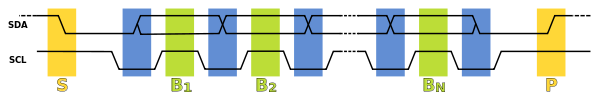
\includegraphics[width=0.7\linewidth]{i2cclock}
		\caption{Listing szyny
			\cite{image:i2c}}
		\label{fig:i2cclock}
	\end{figure}
}


\frame{
	\frametitle{USB}
	Stosowana do połączeń Plug and Play urządzeń zewnętrznych komputera.
	\begin{itemize}
		\item 5 m
		\item 127 urządzeń
	\end{itemize}
	\begin{itemize}
		\item v2.0 -> 480Mbit/s; 500 mA
		\item v3.2 -> 20Gbit/s; 900 mA 
		\item USB-C; 3 A
		\item OMTP/GSMA; 1.5 A
		\item Pojedynczy host odpytuje wszystkie urządzenia cyklicznie
	\end{itemize}
	
	\begin{itemize}
		\item Koncentratory
		\item Bezprzewodowy USB
	\end{itemize}
}

\frame{
	\frametitle{USB}
	\begin{figure}
		\centering
		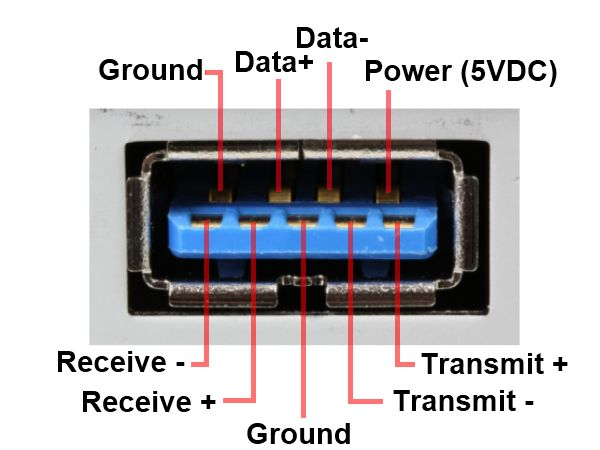
\includegraphics[width=0.9\linewidth]{usb3pinout}
		\caption{Złącze USB v3 typ A
			\cite{image:usbpinout}}
		\label{fig:usb3pinout}
	\end{figure}
}

\frame{
	\frametitle{USB}
	\begin{figure}
		\centering
		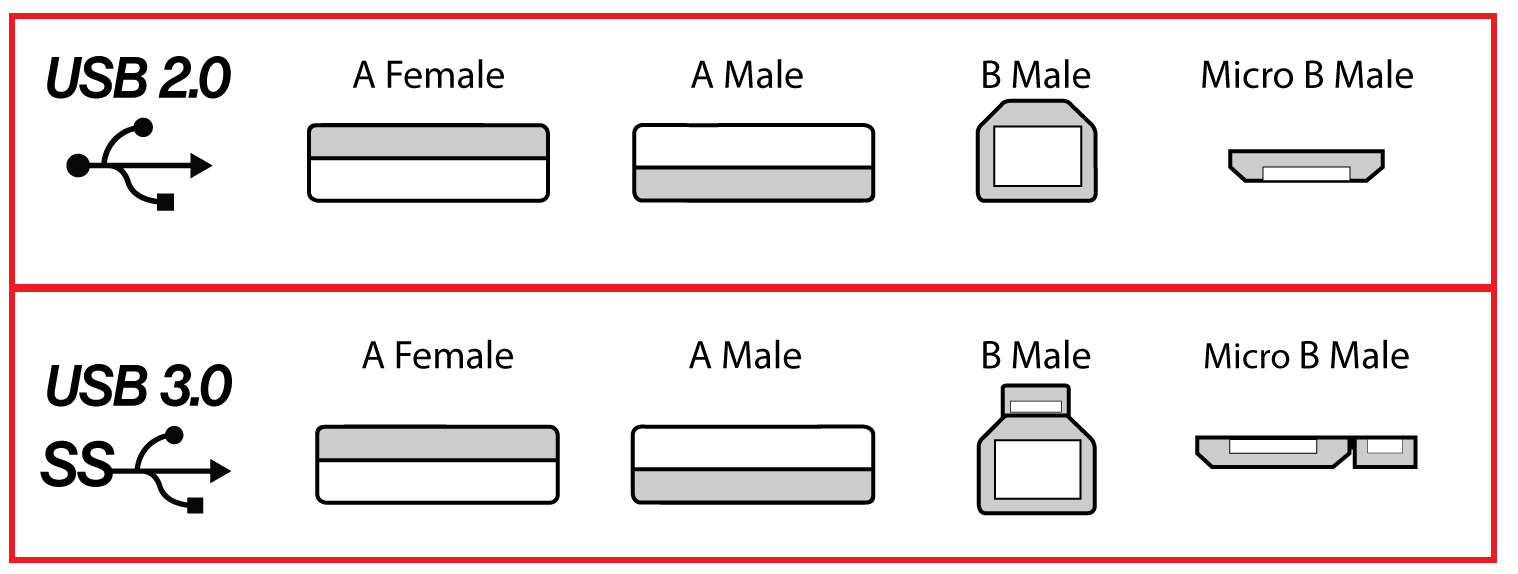
\includegraphics[width=0.9\linewidth]{usbconnectors}
		\caption{Złącza USB
			\cite{image:usbconnectors}}
		\label{fig:usbconnectors}
	\end{figure}
	\begin{figure}
		\centering
		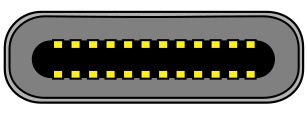
\includegraphics[width=0.3\linewidth]{usb3c}
		\caption{Złącze USB C
			\cite{image:usbconnectors}}
		\label{fig:usb3c}
	\end{figure}
	}

\frame{
	\frametitle{100BASE-TX}
	\begin{itemize}
		\item 100 m
		\item 100 Mbit/s
		\item Dwie pary różnicowe (cztery przewody nieużywane)
		\item Topologia gwiazdy (switche)
		\item CSMA/CD -> sygnał JAM
		\item Transformatory 1:1 (separacja poziomu odniesienia)
		\item Power over Ethernet -> do 60 V; do 400 mA
	\end{itemize}
}
\frame{\frametitle{10GBASE-T}
	\begin{itemize}
		\item F = 500MHz
		\item Przesunięte pary różnicowe
		\item Separacja par różnicowych
		\item Kable kat. 6 (55 m) oraz 6a (100 m)
	\end{itemize}
	
	\begin{figure}
		\centering
		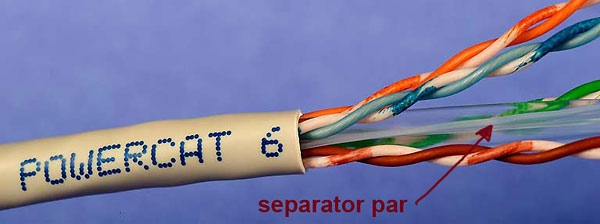
\includegraphics[width=0.9\linewidth]{ethernet6}
		\caption{Kabel skrętkowy kat. 6
			\cite{ethernet}}
		\label{fig:ethernet6}
	\end{figure}
}

\frame{\frametitle{Ethernet}
	\begin{figure}
		\centering
		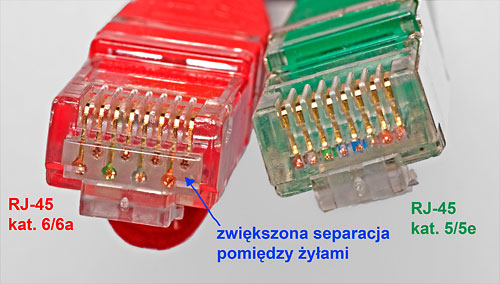
\includegraphics[width=0.9\linewidth]{ethernetzlacza}
		\caption{Wtyki RJ-45
			\cite{ethernet}}
		\label{fig:ethernetzlacza}
	\end{figure}
}

\frame{
	\frametitle{100BASE-Tx}
		\begin{figure}
			\centering
			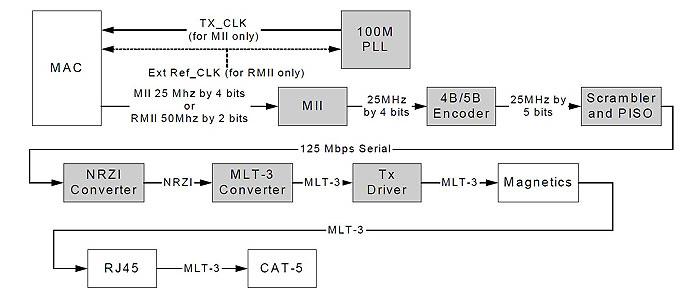
\includegraphics[width=0.9\linewidth]{ethernetflow}
			\caption{Przepływ danych w karcie sieciowej
				\cite{ethernet}}
			\label{fig:ethernetflow}
		\end{figure}
}
\frame{
	\frametitle{100BASE-Tx}
	\begin{figure}
		\centering
		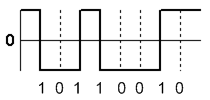
\includegraphics[width=0.5\linewidth]{nrzi}
		\caption{Kod NRZI
			\cite{image:nrzi}}
		\label{fig:nrzi}
	\end{figure}
	
	\begin{figure}
		\centering
		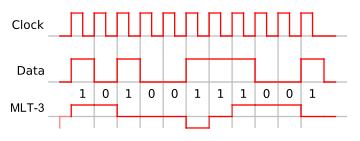
\includegraphics[width=0.5\linewidth]{mlt3}
		\caption{Kod MLT-3
			\cite{image:mlt3}}
		\label{fig:mlt3}
	\end{figure}
}


\frame{\frametitle{WiFi}
	\begin{itemize}
		\item ok. 100-200 m
		\item 2,4 GHz lub 5,8 GHz
		\item B, G, N, AC
		\item (Half-duplex)
		\item Nie wszystkie urządzenia się widzą
		\item CSMA/CA -> synał próbny
		\item Kanały
	\end{itemize}
}


\frame{\frametitle{UDP i TCP}
	UDP:
	\begin{itemize}
		\item Szybki
		\item Brak potwierdzenia odbioru
		\item CRC
	\end{itemize}
	TCP:
	\begin{itemize}
		\item Wolniejszy
		\item Niezawodny
		\item Algorytm Neagle'a
		\item Szatkowanie danych
		\item Niepewność kolejności otrzymania
	\end{itemize}
}

\frame{
	\frametitle{Modbus TCP/IP}
	\begin{figure}
		\centering
		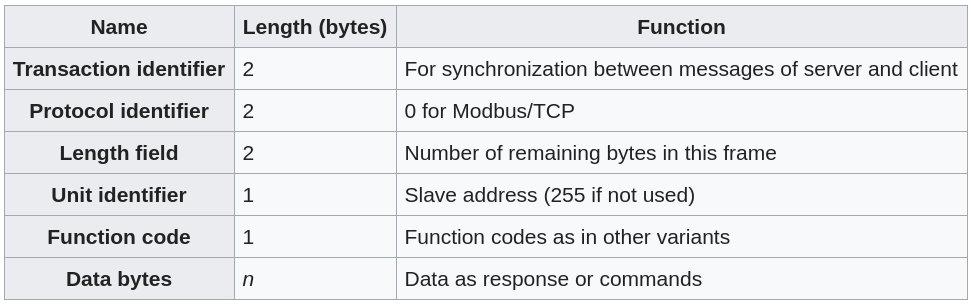
\includegraphics[width=0.9\linewidth]{modbusramka}
		\caption{Instrukcje protokołu dla TCP/IP
			\cite{image:modbus}}
		\label{fig:modbusramka}
	\end{figure}	
}

\frame{
	\frametitle{Ethercat}
	\begin{itemize}
		\item Wykorzystuje np. 100BASE-Tx
		\item Prędkości rzędu kilku kH 
		\item Jeden master
		\item Węzły slave to wyspecjalizowane urządzenia
		\item Jitter < 1 us
		\item Dowolna topologia (najpopularniejsza szeregowa)
		\item W każdym cyklu master inicjuje przesyłanie ramki przechodzącej przez wszystkie węzły
		\item Ciągła synchronizacja czasu
		\item PDO synchroniczne i asynchroniczne
		\item Broadcast
		\item CoE, EoE, DS 301, ...
	\end{itemize}
}


\frame{\frametitle{Serwonapęd}
	\begin{itemize}
		\item Ehtercat lub światłowód
		\item Połączenie z enkoderami (pary różnicowe)
		\item Stopień mocy
		\item Wejścia cyfrowe
		\item Wyjścia cyfrowe
	\end{itemize}
	\begin{figure}
		\centering
		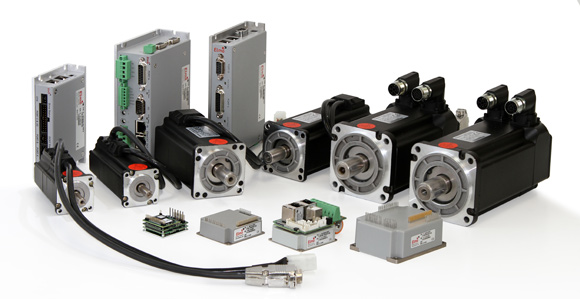
\includegraphics[width=0.9\linewidth]{elmo}
		\caption{Serwonapędy i silniki}
		\label{fig:elmo}
	\end{figure}	
	
	}
	
\frame{	
	\frametitle{IRp-6}
	\begin{figure}
		\centering
		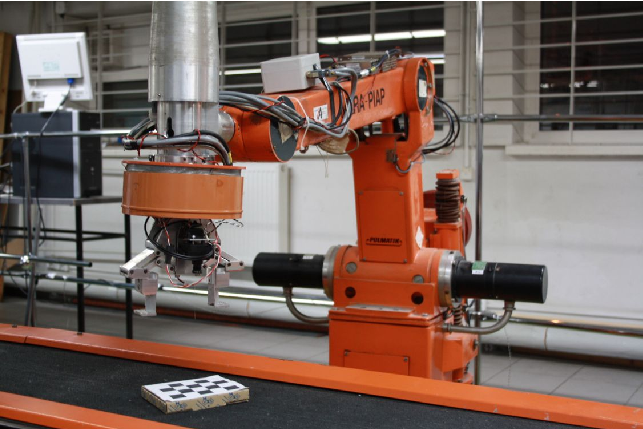
\includegraphics[width=0.9\linewidth]{irpcaly}
		\caption{Robot IRp-6}
		\label{fig:irpcaly}
	\end{figure}	
	}
\frame{
	\frametitle{IRp-6}
		\begin{itemize}
			\item RTLinux
			\item Orocos
			\item ROS
		\end{itemize}
		\begin{itemize}
			\item EtherCAT
			\item CAN
			\item RS-485
			\item Interfejsc A/C i C/A
			\item Szyny zasilające
		\end{itemize}
}

\frame{
	\frametitle{Czujnik siły}
	\begin{itemize}
		\item Zasilanie -15 V; +15 V
		\item Zasilanie 5 V
		\item Analogowy sygnał opisujący pomiar siły
		\item Multiplekser wybierający kanał pomiaru
	\end{itemize}
		\begin{figure}
			\centering
			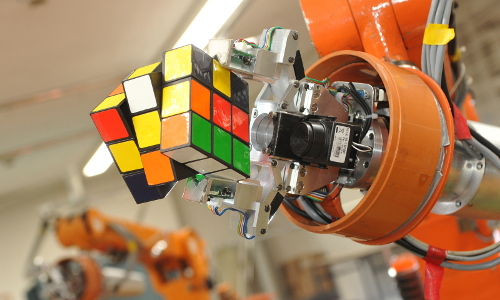
\includegraphics[width=0.6\linewidth]{irp}
			\caption{Chwytak robota IRp-6}
			\label{fig:irp6}
		\end{figure}
}

\frame{\frametitle{Co zrobiliśmy źle?}
		\begin{figure}
			\centering
			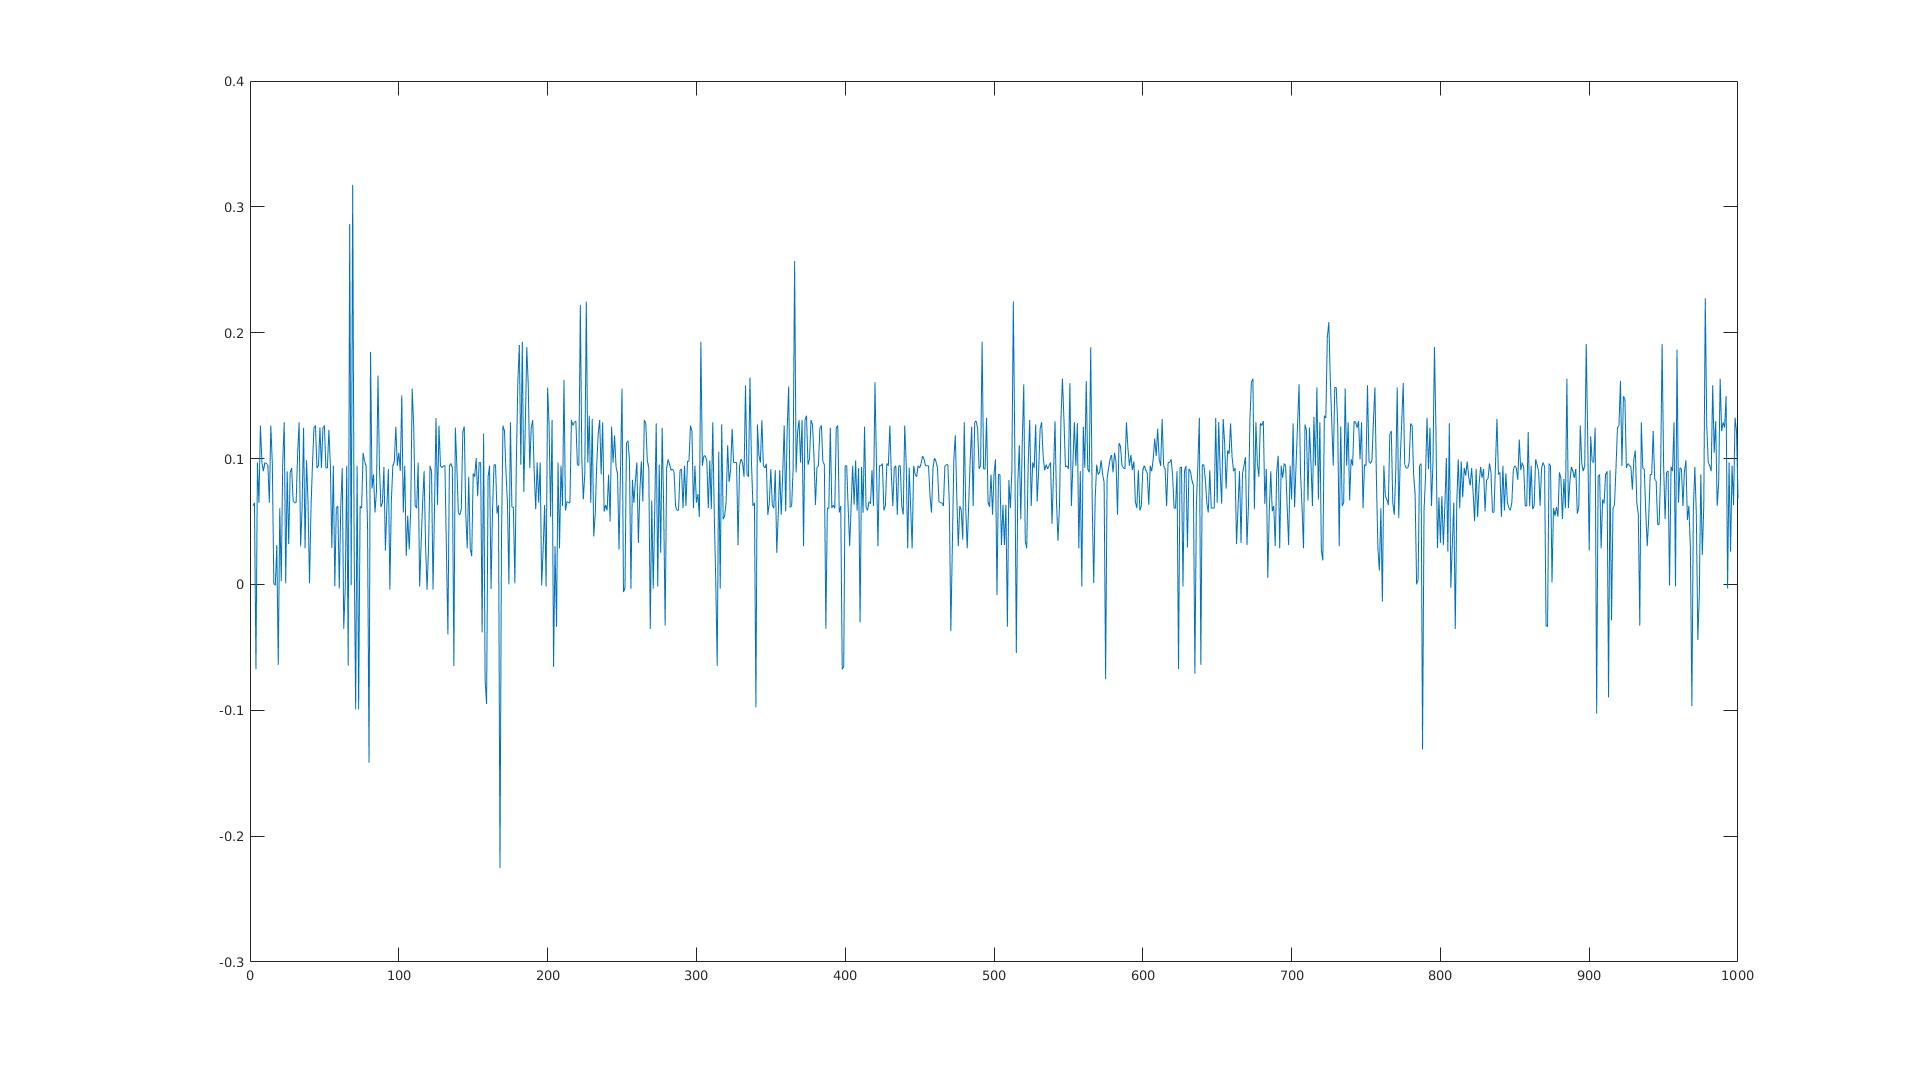
\includegraphics[width=1.1\linewidth]{czujniksily}
			\caption{Odczyt siły w osi X}
			\label{fig:czujniksily}
		\end{figure}
	}
	
\frame{\frametitle{Jak to poprawić?}
	\begin{figure}
		\centering
		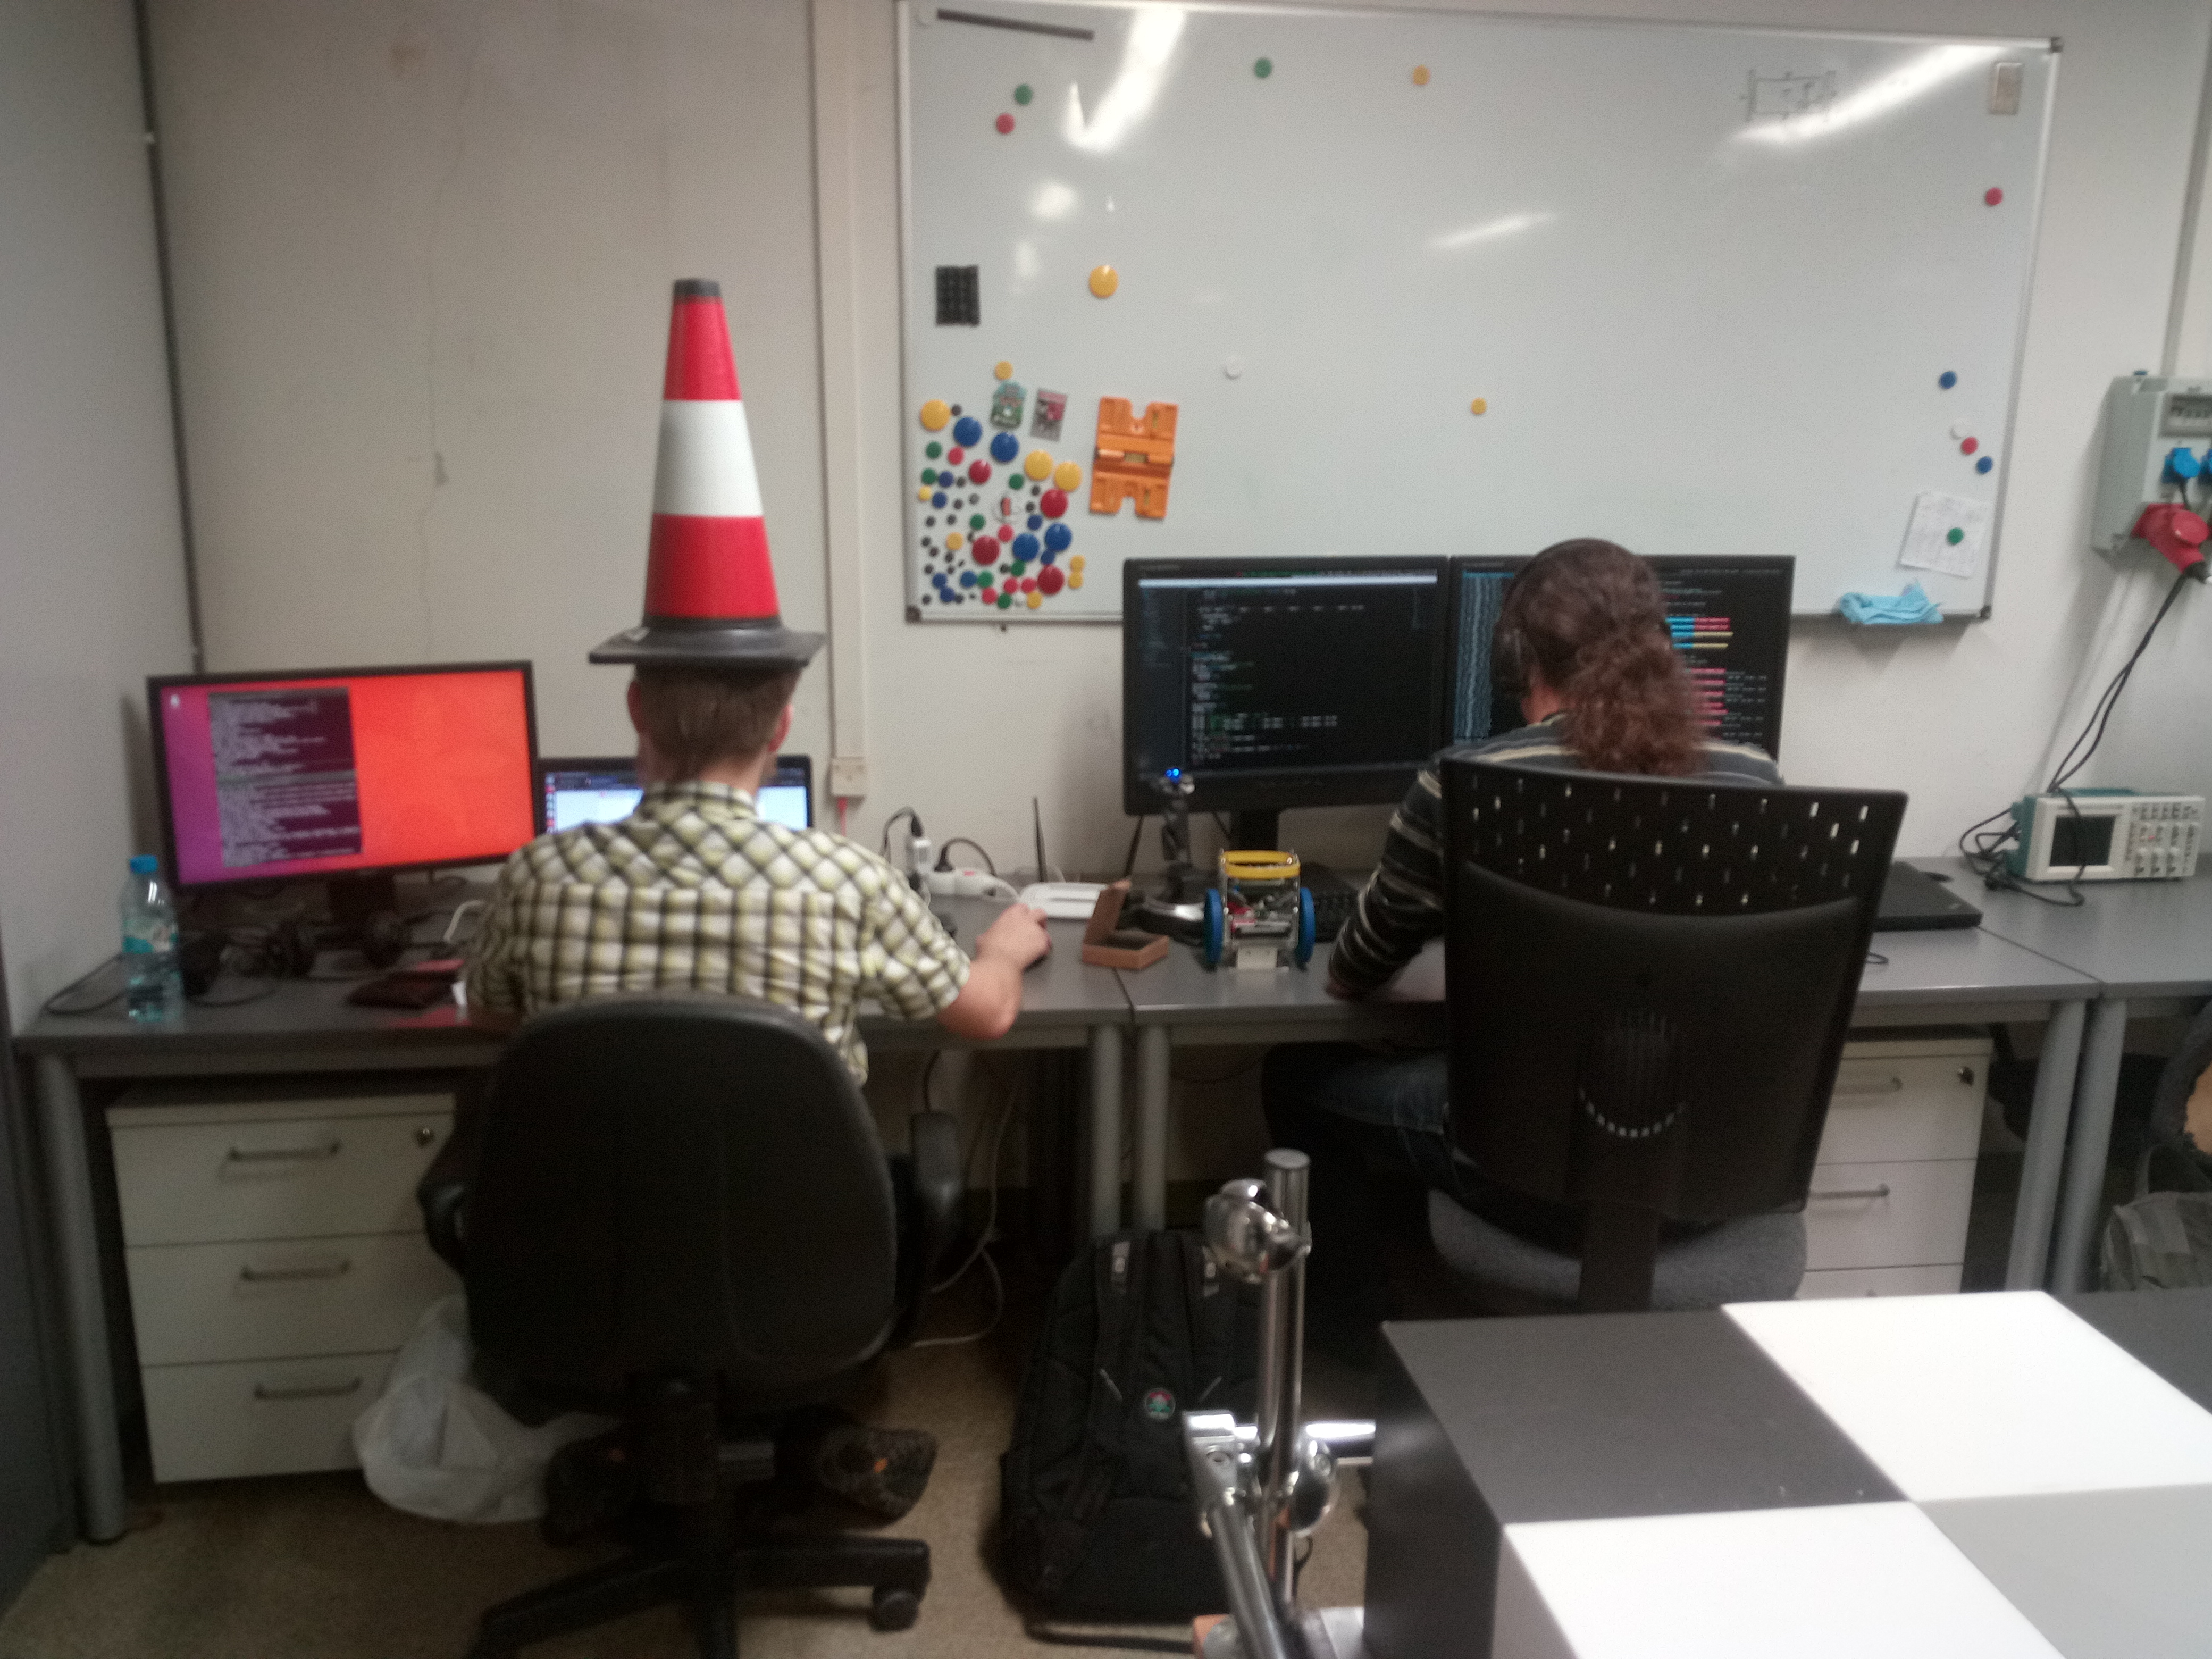
\includegraphics[width=0.85\linewidth]{daniel}
		\caption{Dwóch studentów męczących się dopiero drugi semestr z pracą inżynierską. Zdjęcie poglądowe.}
		\label{fig:daniel}
	\end{figure}
}

\frame{\frametitle{Za chwilę dalszy ciąg programu}
	\begin{itemize}
		\item Hyper Transport
		\item Gigavision
		\item NFC
		\item Wireless Sensor Network
		\item Telekomunikacja
		\item RTOS
		\item Sterowniki urządzeń
		\item Bezpieczeństwo
		\item ROS
	\end{itemize}
}

\begin{frame}[allowframebreaks]{Bibliografia}
\bibliographystyle{plain}
\bibliography{bibliography}
\end{frame}

\frame{\frametitle{Dziękuję za uwagę}
	\begin{figure}
		\centering
		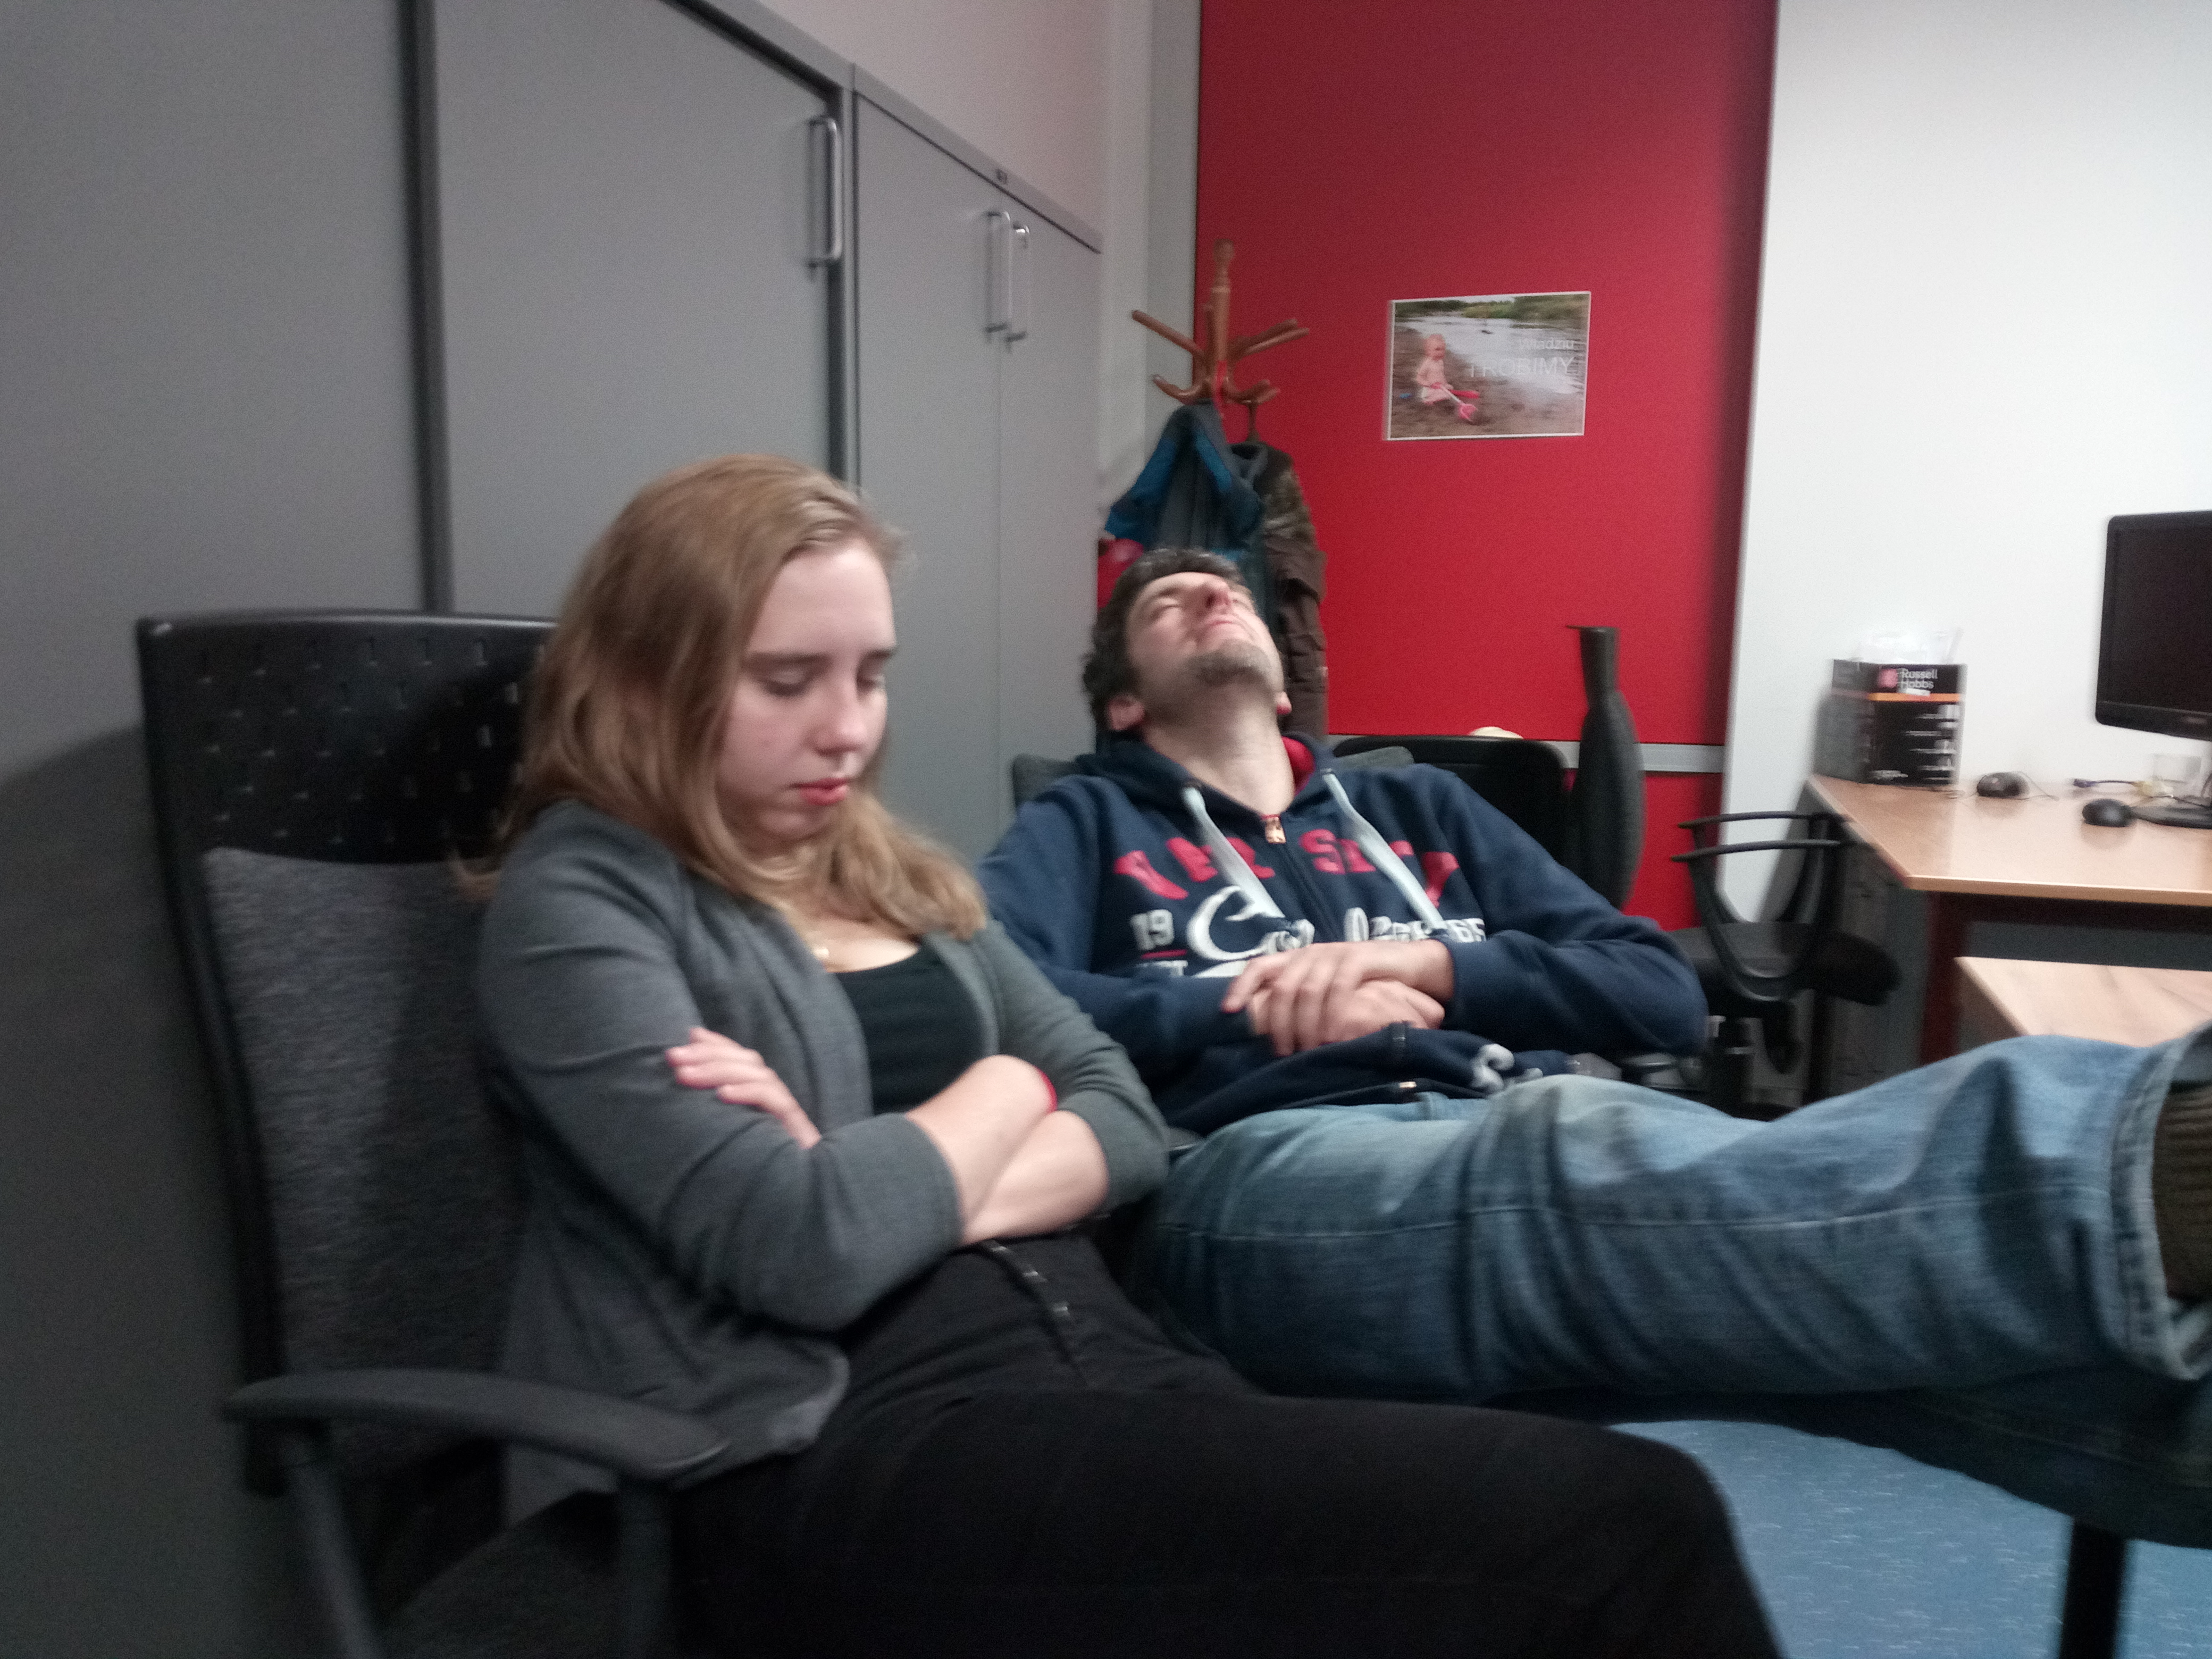
\includegraphics[width=0.9\linewidth]{karolina}
	\end{figure}}

\end{document}
